% MA211 - Lecture 18
\documentclass[pdftex, xcolor=pdftex, dvipsnames]{beamer}

\usetheme{MA211}
\usepackage{thumbpdf}
\usepackage{wasysym}
%\usepackage{ucs}
\usepackage[utf8]{inputenc}
\usepackage{pgf,pgfarrows,pgfnodes,pgfautomata,pgfheaps,pgfshade}
\usepackage{verbatim}

\usepackage{eurosym}
\usepackage{euler}

\usepackage{calc}               % Simple computations with LaTeX variables
%\usepackage[hang]{caption2}     % Improved captions

\usepackage{graphicx}           % Standard graphics package

\usepackage{amsmath, amsthm, amssymb}


\newcommand{\fquad}{\mbox{\qquad}}
\newcommand{\bull}{$\bullet$ }

\newcommand {\I} {\mathcal I}
\newcommand {\calI} {\mathcal I}
\def\disint{\displaystyle\int}

\DeclareMathOperator{\D}{d}
\newcommand{\dydx}{\frac{\D y}{\D x}}

%\definecolor{gray}{rgb}{0.69, 0.69, 0.69} \newcommand{\gray}[1]{\textcolor{gray}{#1}}
\definecolor{dogreen}{rgb}{0.33, 0.42, 0.18} \newcommand{\dogreen}[1]{\textcolor{dogreen}{#1}}
\definecolor{maroon}{rgb}{.5,0.2,0.2}\newcommand{\maroon}[1]{\textcolor{maroon}{#1}}
\definecolor{greena}{rgb}{.1,0.581,0.1}\newcommand{\greena}[1]{\textcolor{greena}{#1}}

\definecolor{blue4}{rgb}{0,0,.545}
\newcommand{\Blue}[1]{\textcolor{blue}{#1}}
\newcommand{\Red}[1]{\textcolor{red}{#1}}
\definecolor{pink}{rgb}{1.,0.75,0.8}
\definecolor{darkred}{rgb}{0.5,0.0,0.0}
\definecolor{darkgreen}{rgb}{0,0.3,0.3}
\definecolor{purple}{rgb}{0,0.3,0.3}
\definecolor{darkblue}{rgb}{0.0, 0.0, .5}
\definecolor{dpurple}{rgb}{.3,.0,.3}
\newcommand{\Green}[1]{\textcolor{darkgreen}{#1}}
\newcommand{\DRed}[1]{\textcolor{darkred}{#1}}
\newcommand{\DBlue}[1]{\textcolor{darkblue}{#1}}
\newcommand{\Purple}[1]{\textcolor{dpurple}{#1}}
\newcommand{\Emph}[1]{\textcolor{darkred}{\textbf{\it #1}}}
\newcommand{\remph}[1]{\textcolor{darkred}{\textbf{\emph{#1}}}}
\newcommand{\bemph}[1]{\textcolor{darkblue}{\textbf{\emph{#1}}}}
\newcommand{\gemph}[1]{\textcolor{darkgreen}{\textbf{\emph{#1}}}}
\newcommand{\Bf}[1]{\textcolor{darkblue}{\textbf{#1}}}
\newcommand{\Gf}[1]{\textcolor{darkgreen}{\textbf{#1}}}
\newcommand{\Rf}[1]{\textcolor{red}{\textbf{#1}}}
\newcommand{\Rmf}[1]{\textcolor{red}{\mathbf{#1}}}

\newcommand{\Conj}[1]{\overline{#1}}

\newcommand{\code}[1]{\textcolor{darkblue}{\texttt{\textbf{#1}}}}
\newcommand{\icode}[1]{{\blue\texttt{\textbf{\emph{#1}}}}}
\newcommand{\gcode}[1]{{\Green{\texttt{\textbf{\emph{#1}}}}}}
\newcommand{\out}[1]{\texttt{\emph{\textbf{\Green{#1}}}}}





\newenvironment{vminipage}%
{\begin{Sbox}\begin{minipage}\begin{small}\begin{verbatim}}%
{\end{verbatim}\end{small}\end{minipage}\end{Sbox}\fbox{\TheSbox}}

\newenvironment{nminipage}%
{\begin{Sbox}\begin{minipage}}%
{\end{minipage}\end{Sbox}\fbox{\TheSbox}}


\let\Arg\relax\DeclareMathOperator{\Arg}{\mathtt{Arg}}
\let\Arg\relax\DeclareMathOperator{\e}{\mathtt{e}}

\newcommand {\AND} {\wedge}
\newcommand {\OR} {\vee}
\newcommand {\NOT} {\neg}
\newcommand {\IMPLIES} {\rightarrow}
%\newcommand {\IFF} {\leftrightarrow}
\renewcommand {\iff} {\Leftrightarrow}
\newcommand {\NAND} {\uparrow}
\newcommand {\NOR} {\downarrow}
\newcommand {\XOR} {\otimes}

\newenvironment{citemize}% Colour items
{\begin{description}}%
{\end{description}}

\newcommand {\maroonitem}{\item[\maroon{$\bullet$}]}

\newcommand {\gitem} {\item {\includegraphics[width=.4cm,angle=-10]{img/green-bullet-on-white.ps}}}
\newcommand {\ritem} {\item {\includegraphics[width=.4cm,angle=-10]{img/red-bullet-on-white.ps}}}
\newcommand {\yitem} {\item {\includegraphics[width=.4cm,angle=-10]{img/yellow-bullet-on-white.ps}}}
\newcommand {\bitem} {\item {\includegraphics[width=.4cm,angle=-10]{img/blue-bullet-on-white.ps}}}

\newcommand {\greenitem} {\item {\includegraphics[width=.4cm,angle=-10]{img/green-bullet-on-white.ps}}}
\newcommand {\reditem} {\item {\includegraphics[width=.4cm,angle=-10]{img/red-bullet-on-white.ps}}}
\newcommand {\yellowitem} {\item {\includegraphics[width=.4cm,angle=-10]{img/yellow-bullet-on-white.ps}}}
\newcommand {\blueitem} {\item {\includegraphics[width=.4cm,angle=-10]{img/blue-bullet-on-white.ps}}}

\newcommand {\eq}[1]%
  {$\DBlue{#1}$}
\newcommand {\eqd}[1]%
  {$\displaystyle\DBlue{#1}$}
%\newcommand{\eq}[1]{\boldmath \DBlue{$#1$}}


\newcommand {\csf}{\centerslidesfalse}
\newcommand {\cst}{\centerslidestrue}

\newcommand {\vecii}[2] {   \big(\begin{smallmatrix} #1 \\ #2 \end{smallmatrix}\big)}
\newcommand{\atwo}[2]{\left(\!\!\begin{array}{c} #1 \\ #2 \end{array}\!\!\right)}


\newcommand{\C}{\mathbb{C}}
\newcommand{\Q}{\mathbb{Q}}
\newcommand{\R}{\mathbb{R}}
\newcommand{\N}{\mathbb{N}}
\newcommand{\Z}{\protect\mathbb{Z}}  % protect for index.
\newcommand {\Rs}{ \mathbb{R}}
\newcommand {\Cs}{ \mathbb{C}}
\newcommand {\Rnn}{ \mathbb{R}^{n \times n}}
\newcommand {\Rn}{ \mathbb{R}^{n}}


\newcommand{\mblock}{%
\setbeamercolor*{block title}{bg=maroon,fg=white}
\setbeamercolor*{block body}{bg=white,fg=maroon}
}%

\newcommand{\bblock}{%
\setbeamercolor*{block title}{bg=Steel,fg=white}
\setbeamercolor*{block body}{bg=Mylightgray,fg=Steel}
}%

\newcommand{\gblock}{%
\setbeamercolor*{block title}{bg=Green,fg=white}
\setbeamercolor*{block body}{bg=Mylightgray,fg=darkgreen}
}%


\newcommand{\rblock}{%
\setbeamercolor*{block title}{bg=Red,fg=white}
\setbeamercolor*{block body}{bg=white,fg=Black}
}%


\newcommand{\TakeNotes}{
\includegraphics[width=2cm]{TakeNote}}

\def\eps{\varepsilon}
\newcommand {\del}[2]{ {\frac{\partial #1}{\partial #2}}}
\newcommand {\x}[1]{x^{[#1]}}
\newcommand {\delx}{ {\frac{\partial}{\partial x}}}
\newcommand {\delt}{ {\frac{\partial}{\partial t}}}
\newcommand {\dely}{ {\frac{\partial}{\partial y}}}
\newcommand {\ith}{{(i)}}
\renewcommand {\vec}[1]{ {\boldsymbol{#1}}}



\newcommand {\Rsym}{{ \mathbb{R}^{n \times n}_\mathrm{sym}}}

\newcommand {\st} {\mathrm{st}}
\newcommand {\nd} {\mathrm{nd}}


\parskip .25cm


\theoremstyle{definition}
\newtheorem{exercise}{Exercise}[section]
\newtheorem{method}{Method}[section]

\newcommand{\Header}[1]{\begin{center}{\Large \Bf{#1}}\end{center}}

\subtitle{MA211}
\title{Lecture 18: Integration by parts}

\author{Dr Niall Madden}

\date{\Large Mon $10^\mathrm{th}$ Nov 2008}


\begin{document}

\setcounter{framenumber}{-1}
\frame{

%\begin{columns}[c]
%\column{0.45\textwidth}
%\centering
%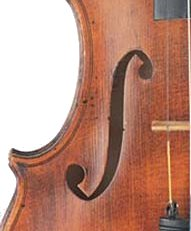
\includegraphics[width=4cm]{images/violin}
%
%
%\column{0.55\textwidth}
\begin{block}{}
\begin{center}
\begin{large}
 \insertsubtitle
\end{large}

\vspace{.1cm}

\begin{Large}
\textbf{\inserttitle}
\end{Large}


\vspace{.3cm}

{\insertdate}

\end{center}
\end{block}


\begin{center}
{\Large \eqd{\int \alert{u} dv = \alert{u}v - \int v \alert{du}}}
\end{center}

% \end{columns}

}



\frame{
  \frametitle{Today...}

%\begin{columns}[c]
%\column{0.5\textwidth}
 \tableofcontents
%\column{0.5\textwidth}


See also Section 7.1 of Stewart.

%\end{columns}
}



\section{Integration by parts}

\frame{

 Recall that if we are differentiating the product of two
  functions $u$ and $v$ then \eqd{\frac{d}{dx}\big(uv) = u
    \frac{dv}{dx} + v \frac{du}{du}}.

Now, using  that\eqd{\int  \frac{d}{dx}\big(uv) dx = uv} we can deduce
the following

\vspace{3cm}

}


\frame{

The most important technique for integrating is:

\begin{block}{}
\Header{Integration by Parts}
\[
\int u dv = uv - \int vdu.
\]
\end{block}

Using this formula, we try to replace the integral with one that is
easier to solve.

\pause

The main ``\emph{trick}'' is in choosing \eq{u} and \eq{dv}.

\pause
Usually we are trying to integrate the product of 2 functions (though
this is not always obvious!).

As a rule of thumb, first try  the one that is easiest to integrate as
\eq{dv}


}

\subsection{$\int u dv = uv - \int vdu.$}
\frame{
\begin{example}[1]
Evaluate \qquad \eqd{\I=\int x e^x dx}.
\end{example}
\pause 
\Bf{Soln: } Let \eq{u=x, \qquad dv = e^x dx}
\vspace{4cm}
}


\frame{
\begin{example}[2]
Evaluate ~~ \eqd{\I = \int x \sin(x) dx}.
\end{example}


\vspace{4cm}
}


\frame{
\begin{example}[3]
Evaluate ~ \eqd{\I = \int \alert{x^2} \sin(x) dx}.
\end{example}
\pause
\Bf{Soln: } Let \eq{u=x^2, \qquad dv = \sin(x) dx}.
\vspace{4cm}
}

\frame{
\begin{example}[4]
(\emph{From Q1 (c) (i), Aut 06/07})\\
Evaluate \qquad  \eqd{\alert{\I}=\int \ln(x) dx}.
\end{example}
\vspace{4cm}
}



\frame{
\begin{example}[5]
(\emph{From Q1 (b), Aut 05/06})\\
Evaluate \eqd{\alert{\I}=\int \tan^{-1}(x)  dx}.
\end{example}
\vspace{4cm}
}

\frame{
\begin{exercise}[18.2]
 Using \emph{Integration by parts}, evaluate the following
  integrals
\begin{enumerate}[(i)]
\item  \eqd{\int x \cos(x) dx}.
\item \eqd{\int \big(\ln(x)\big)^2 dx}.
\item  \eqd{\int x \tan^{-1}(x)  dx}.
\item \eqd{\int x^2 \tan^{-1}(x)  dx}.
\item \eqd{\int (x+3) e^{2x} dx}.
\end{enumerate}


\end{exercise}

}


\subsection{Definite Integrals}

\frame{

\begin{block}{}
\Header{Integration by Parts for Definite Integrals}
\[
\int_a^b u dv = uv\bigg|_a^b - \int_a^b vdu.
\]
\end{block}

}

\frame{

\begin{example}[6]
Use that \eqd{\int_a^b u dv = uv\bigg|_a^b - \int_a^b vdu}
to evaluate 
\eqd{\int_1^2  \frac{\ln(x)}{x} dx}
\end{example}
\vspace{4cm}

}


\frame{

\begin{example}[7]
Use that \eqd{\int_a^b u dv = uv\bigg|_a^b - \int_a^b vdu}
to evaluate 
\eqd{\int_1^e x^3 \ln (x) dx}
\end{example}
\vspace{4cm}

}


\frame{
\begin{exercise}[18.3]

Evaluate the following definite integrals
\begin{enumerate}[(i)]
\item \eqd{\int_1^2 \ln(x) dx}
\item  \eqd{\int_1^2 \frac{\ln(x)}{x} dx}
\item  \eqd{\int_{\pi/6}^{\pi/2} \frac{x}{\sin^2(x)} dx}.\\ ~~ \emph{Hint:
    if $f(x) = \displaystyle\frac{\cos(x)}{\sin(x)}$, what is $f'(x)$?}
\end{enumerate}



\end{exercise}
}



\section{Reduction Formulae}

\frame{

We'll now have a look at how to use integration by parts:
\begin{block}{}
\Header{Integration by Parts}
\[
\int u dv = uv - \int vdu,
\]
\end{block}

to  to replace an integral... with itself!
Surprisingly, this turns out to be useful.


}




\frame{

Some times we can use integration by parts twice:
\begin{example}[1]
Show that \eqd{\int e^x \cos(x) dx = \frac{1}{2}\big(e^x \sin(x) + e^x
  \cos(x)\big) + C}.
\end{example}

\vspace{4cm}
}


\frame{
\begin{example}[2]

Show that
\[
\int sin^n(x) dx = - \frac{1}{n} \cos(x) sin^{n-1}(x) + 
\frac{n-1}{n} \int sin^{n-2}(x) dx.
\]
\end{example}
\vspace{4cm}

}

\frame{

\begin{exercise}[Q18.4]
 Using \emph{Integration by parts to answer the following
    questions}
\begin{enumerate}[(i)]
\item Evaluate \eq{\int x^2 e^x dx}.

\item Evaluate \eq{\int x^5 e^{x^2} dx}. (\emph{Hint: first use a
    substitution, then use the answer to part (i)}).

\item Evaluate \eq{\int e^x \sin(x) dx}.

\item Let \eqd{\I_n = \int_0^1 x^n e^x dx}. Show that \eqd{\I_n + n
    \I_{n-1} = e}.

\item  Evaluate \eqd{\int \sin\big(\ln(x)\big) dx}.
\end{enumerate}
\end{exercise}
}


\section{Partial Fractions}
\frame{

Suppose we want to evaluate the integral of 
\eqd{\frac{x+4}{x^2 - 5x + 6}}.

We know that we can write
\[ 
\frac{x+4}{x^2 - 5x + 6}
=
\frac{x+4}{(x-2)(x-3)}
\]
and that this can be further simplified using \Emph{partial
  fractions:}

\vspace{2cm}
}




\frame{
\begin{example}[1]
Evaluate \eqd{\int \frac{1}{x(x^2+1)}  dx}.
\end{example}
\vspace{4cm}
}

\frame{
\begin{exercise}[Q18.5]
 Evaluate the following:
\begin{enumerate}[(i)]
\item \eqd{\int \frac{1}{x(x^2-1)}dx}
\item \eqd{ \int \frac{x^3+2}{x^3-1} dx}
\item \eqd{\int \frac{2x+1}{x^2 + 4x +\mathbf{4}}dx}
\item \eqd{\int_2^3 \frac{3x^3+1}{x^3 -2x^2 +x}dx}
\end{enumerate}
\end{exercise}

}

\end{document}
\section{Proper Integrals}

\frame{

So far, the definite integrals we have considered:
\[  \int_a^b f(x) dx, \]
have all been \Emph{Proper}: they are integrals of bounded functions
on closed, finite intervals. 
\pause
\begin{columns}
\column{0.6\textwidth}
\begin{center}
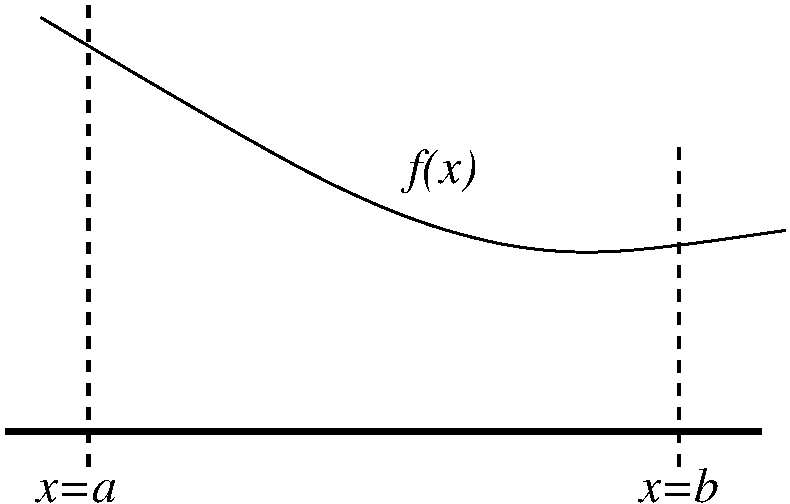
\includegraphics[width=6cm]{Proper}
\end{center}
\column{0.4\textwidth}
So we when we think of the integral as the area between the graph of
the function and the \eq{x}-axis, it is clear that that is
well-defined.
\end{columns}

}

\section{Improper Integrals}

\frame{
A definite integral \eqd{\int_a^b f(x) dx} is \Emph{Improper} if:


\begin{block}{\bf{Type I:} if $a = - \infty$ or $b= \infty$}
\begin{center}
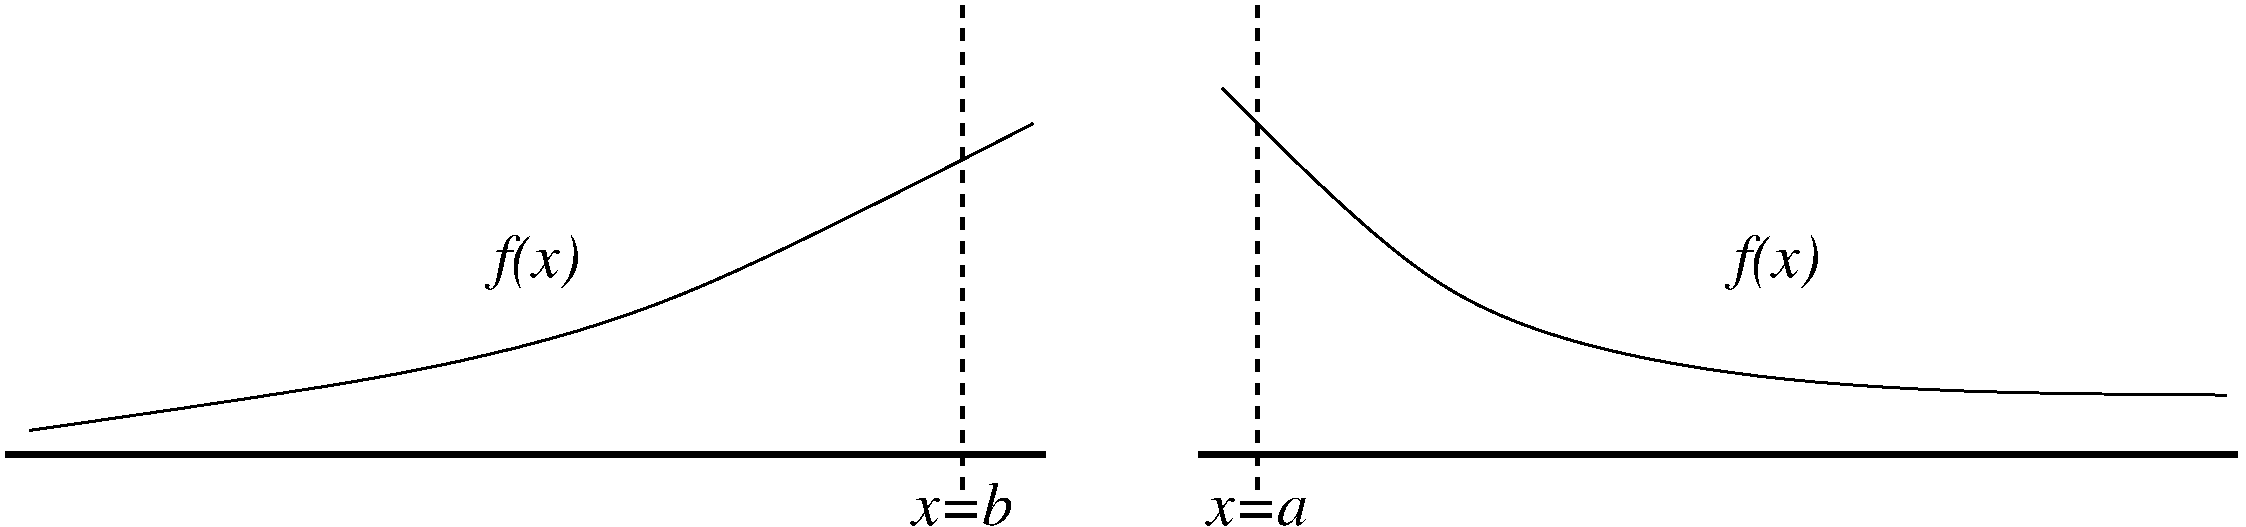
\includegraphics[width=9cm]{Improper1}
\end{center}
\end{block}


\begin{block}{\bf{Type II:} if $f(x)$  is unbounded (infinite) near $a$ or $b$.}
\begin{center}
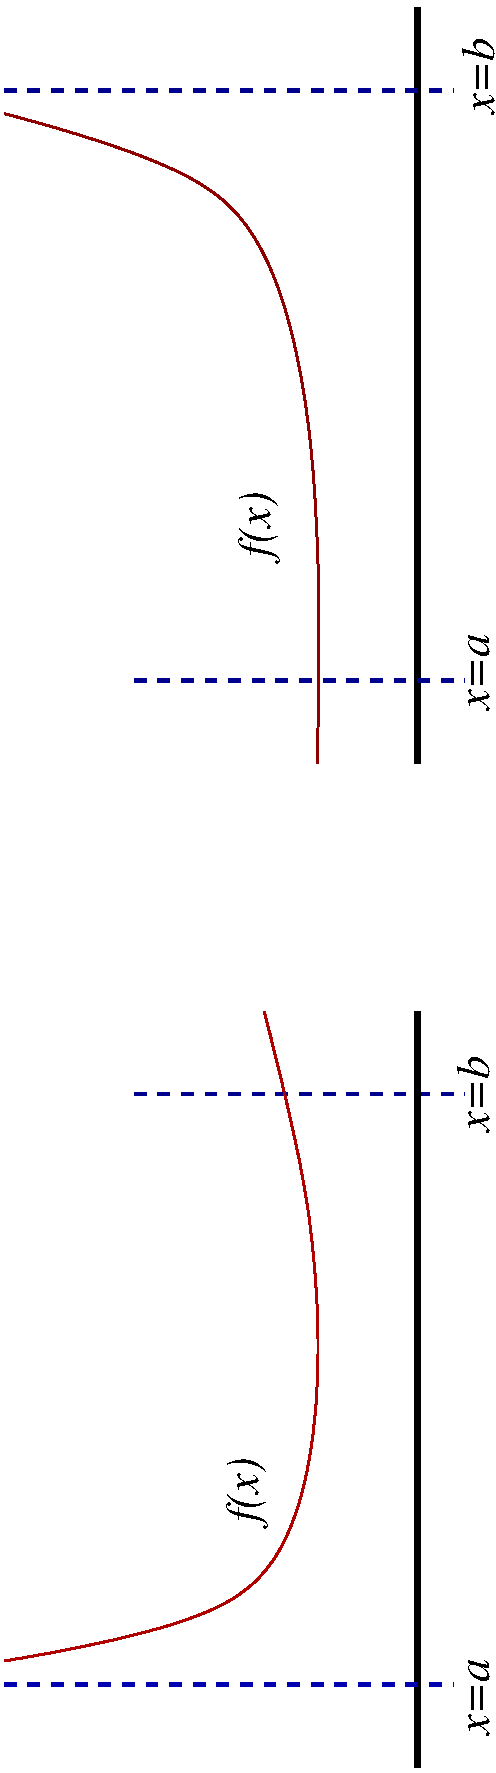
\includegraphics[width=4cm]{Improper2}
\end{center}
\end{block}


}

\frame{

\begin{itemize}
\item \Emph{Some} improper integrals evaluate as a real, finite
  number.  These are are said to \Bf{converge}, or to be
  \Emph{convergent} or \Bf{to exist}.  

\item Those that don't evaluate to a finite number are said to
  \Bf{diverge}, 
or to be \Emph{divergent} or \Bf{not to exist}.
\end{itemize}
}

\section{Improper Integrals of Type I} 
\frame{

\Bf{Improper Integrals of Type I } are of the form
\[ \int_{a}^{\infty} f(x)\,dx \quad  \text{ or } \quad
\int_{-\infty}^{b} f(x)\,dx.
\]
\begin{center}
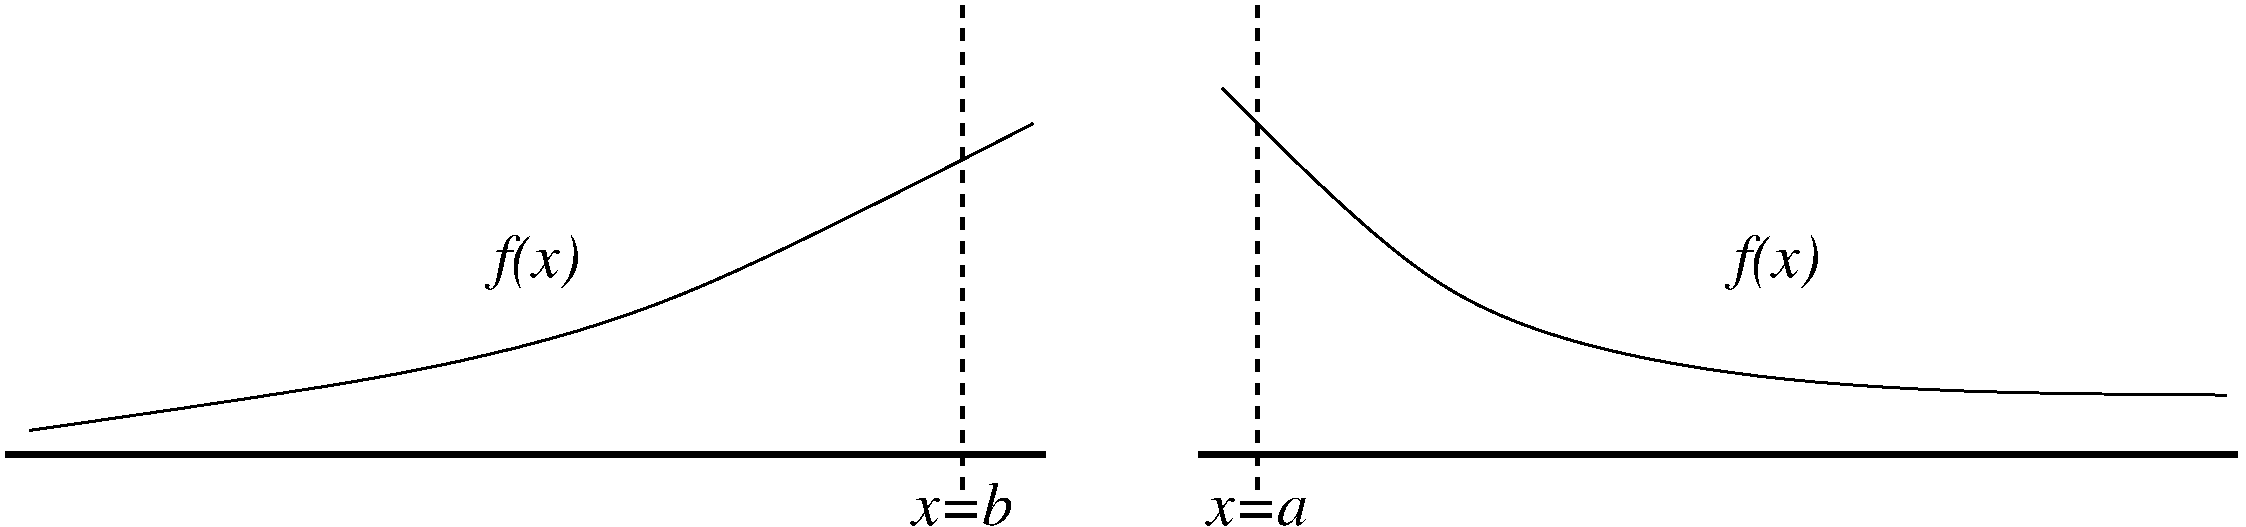
\includegraphics[width=9cm]{Improper1}
\end{center}

To evaluate these, note that \eqd{\int_a^\infty f(x) dx = \lim_{t = \infty}
\int_a^t f(x) dx}. So:
\begin{block}{}
\begin{itemize}
\item Evaluate \eqd{{\cal{I}}(t) = \int_a^t f(x) dx}; 
\item and then compute
\eqd{\lim_{t = \infty} \calI(t)}. 
\end{itemize}
\end{block}
}
\subsection{$\int_a^\infty f(x) dx$}


\frame{
\Header{\eqd{\int_a^\infty f(x) dx}}
\begin{block}{}
\begin{enumerate}
\item Evaluate \eqd{{\cal{I}}(t) = \int_a^t f(x) dx}; 
\item and then compute
\eqd{\I = \lim_{t = \infty} \calI(t)}. 

\item If the limit  exists, call it $L$ and write $\int_{a}^{\infty} f(x)\,dx = L$.
We say that $\int_{a}^{\infty} f(x)\,dx$ {\bf converges to $L$}.

\item  If no such limit exists, $\int_{a}^{\infty} f(x)\,dx$ is said to {\bf diverge}.

\end{enumerate}
\end{block}
}

\frame{

\begin{example}[4]
Evaluate \eqd{\I = \int_{1}^{\infty} \frac{1}{x^2}dx}
\end{example}
\vspace{4cm}
}

\frame{
\begin{example}[5]
Evaluate the improper integral \eqd{\I = \int_{1}^{\infty} \frac{dx}{x}}
\end{example}
\vspace{4cm}
}

\frame{
\begin{example}[6]
Evaluate \eqd{\I = \int_{1}^{\infty} \frac{1}{\sqrt{x}}dx}
\end{example}
\vspace{4cm}
}

\end{document}
\subsection{$ \int_1^\infty{1}/{x^p} dx$}


\frame{
\begin{block}{The general case}
\eqd{\int_{1}^{\infty} 1/x^{p}\,dx}  converges for \eq{p>1}, and
diverges for \eq{p\leq 1}.
\end{block}
\Bf{Proof:}
\vspace{4cm}

}

\frame{
\begin{center}
\includegraphics[width=8cm]{xp}
\end{center}
}

\frame{
\begin{center}
\includegraphics[width=8cm]{xp_int}
\end{center}
}


\frame{
\rblock
\begin{exercise}%[Q2 (b) (i) ,Winter '06]
Test for convergence of the following integral:
\eqd{\int_1^{\infty} \frac{1}{\ln(e^x)}dx}.
\end{exercise}

\vspace{.3cm}

\begin{exercise}[Q2 (b) (vi), Autumn  05/06]
Show that \eqd{\int_0^{\infty} \frac{x^2}{1+x^2}dx}.
\end{exercise}
}


\frame{
\begin{example}[7]
Evaluate the integral $\displaystyle\int_{1}^{\infty} \frac{1}{1+x^2}\alert{dx}$
\end{example}
\vspace{4cm}
}

\subsection{$\int_{-\infty}^b f(x)dx$}

\frame{
For problems of the form
\Header{\eqd{\int_{-\infty}^b f(x) dx}}
\begin{block}{}
\begin{enumerate}
\item Evaluate \eqd{{\cal{I}}(t) = \int_t^b f(x) dx}; 
\item and then compute
\eqd{\I = \lim_{t = -\infty} \calI(t)}. 

\item If the limit  exists, call it $\I$ and write $\int_{-\infty}^b f(x)\,dx = L$.
We say that the integral {\bf converges to $L$}.
\item  If no such limit
exists, it is said to {\bf diverge}.

\end{enumerate}
\end{block}
}



\frame{
\begin{example}[8]
Evaluate $\displaystyle\int_{-\infty}^{-1} \frac{dx}{x^2}$
\end{example}
\vspace{4cm}
}

\frame{
\begin{example}[8]
Evaluate $\displaystyle\int_{-\infty}^{0} e^x dx$
\end{example}
\vspace{4cm}
}


\end{document}
{\sf Integrals of the form} $$\int_{a}^{b} f(x)\,dx$$ where $f(x)$
is unbounded.\\[1cm]
If a function $f$ is defined on $(a,b]$ and $\lim_{t \rightarrow
a^+} \int_{t}^{b} f(x)\,dx$ exists, call it $l$ and write
$\int_{a}^{b} f(x)\,dx = l$. We say that $\int_{a}^{b} f(x)\,dx$
{\bf converges to $l$}. Otherwise, the integral is said to
diverge.

Similarly, if $f$ is defined on $[a,b)$ and $\lim_{t \rightarrow
b^-} \int_{a}^{t} f(x)\,dx$ exists, call it $l$ and write
$\int_{a}^{b} f(x)\,dx = l$. Again, $\int_{a}^{b} f(x)\,dx$ is
said to {\bf converge to $l$}. If no such limit exists, the
integral is divergent. \\[.5cm]
{\sf Examples}
\begin{enumerate}
\item $\displaystyle\int_{0}^{1} \frac{dx}{x}$ \\[3cm]
\item $\displaystyle\int_{0}^{1} \frac{dx}{x^2}$ \\[3cm]
\item $\displaystyle\int_{0}^{1} \frac{dx}{\sqrt{x}}$\\[3cm]
\item {\sf The general case}: $\int_{0}^{1} 1/x^{p}\,dx$ converges for $p < 1$, diverges for $p\geq 1$.\\[1cm]
{\sf Proof}\\[7cm]
\item $\displaystyle\int_{0}^{4} \frac{dx}{\sqrt{4-x}}$ \\[3cm]
\end{enumerate}
{\sf Integrals of the form} $$\int_{-\infty}^{\infty} f(x)\,dx$$
are said to converge if and only if   $\int_{-\infty}^{0}
f(x)\,dx$ and $\int_{0}^{\infty} f(x)\,dx$ {\em both} converge. We
then set $\int_{-\infty}^{\infty} f(x)\,dx = l + m$ where
$\int_{-\infty}^{0} f(x)\,dx= l$ and $\int_{0}^{\infty} f(x)\,dx =
m$.\\[.5cm]
{\sf Example} \\[.5cm]
Show that $\displaystyle\int_{-\infty}^{\infty} \frac{dx}{1 + x^2} = \pi$ \\[3cm]
If a function $f$ is defined on $[a,b]$ except at some point $c$
in $(a,b)$ at which $f$ is {\em unbounded}, then $\int_{a}^{b}
f(x)\,dx$ is said to converge if and only if $\int_{a}^{c}
f(x)\,dx$ and $\int_{c}^{b} f(x)\,dx$ {\em both} converge.\\[.5cm]
{\sf Examples}
\begin{enumerate}
\item $\displaystyle\int_{-1}^{1} \frac{dx}{x}$ \\[3cm]
\item $\displaystyle\int_{-1}^{1} \frac{dx}{\sqrt[3]{x}}$\\[3cm]
\end{enumerate}
It is often difficult to determine the convergence or divergence
of a given integral by direct methods, but we can usually gain
some information by comparison with integrals of known
behaviour.\\[.5cm]
{\sf Comparison Test}\\
Suppose $f$ and $g$ are defined on $[a, \infty)$ and $0 \leq f(x)
\leq g(x) \forall x \in [a, \infty)$. Then
\begin{enumerate}
\item if $\int_{a}^{\infty} g(x)\,dx$ converges, so does
$\int_{a}^{\infty} f(x)\,dx$
 \item if $\int_{a}^{\infty} f(x)\,dx$ converges, so does $\int_{a}^{\infty} g(x)\,dx$
 \end{enumerate}
 Note: We have a corresponding test for improper integrals $\int_{a}^{b}
 f(x)\,dx$ where $f$ is unbounded at $a$.\\[.5cm]
 {\sf Examples}
 \begin{enumerate}
 \item $\displaystyle\int_{1}^{\infty} \frac{x^2\,dx}{ x^2 + x^3}$
 \\[3cm]
 \item $\displaystyle\int_{1}^{\infty} \frac{dx}{x^2 + x^3}$
 \\[3cm]
 \item $\displaystyle\int_{0}^{1}\frac{dx}{ x + x^2}$ \\[3cm]
 \item $\displaystyle\int_{0}^{1}\frac{dx}{ 2x^2 + 3x^3}$
 \\[3cm]
 \item $\displaystyle\int_{0}^{1}\frac{dx}{ 2\sqrt{x} + x^2}$
 \\[3cm]
 \item $\displaystyle\int_{1}^{\infty}\frac{\cos x\,dx}{ 1 + x^2}$
 \\[3cm]
 \end{enumerate}

\end{document}

\end{document}


